% SSAC27 abstract submission. Upload figs/ and this file to Overleaf; compile with pdfLaTeX.
% Rules: under 500 words incl. title, max 2 tables/figures combined, sections Introduction /
% Methods / Results / Conclusion, repo link required. Word count: see wc note in chat.
\documentclass[11pt]{article}
\usepackage[margin=1in]{geometry}
\usepackage{booktabs}
\usepackage{graphicx}
\usepackage[hidelinks]{hyperref}
\usepackage{titlesec}
\titleformat{\section}{\normalfont\large\bfseries}{}{0em}{}
\titlespacing*{\section}{0pt}{8pt}{3pt}
\setlength{\parindent}{0pt}\setlength{\parskip}{4pt}

\title{Conditional Queries Against a Learned Hitter Process Model}
\author{Nate Seluga\\ Harvey Mudd College}
\date{}

\begin{document}
\maketitle
\vspace{-2em}

\section{Introduction}
In baseball, understanding how to use great hitters is often a simple task: play as many of them as you can and play them often. Teams try to gain an edge with the remaining hitters, but less playing time means thinner data in an area that takes hundreds of plate appearances to stabilize. This paper asks whether a model trained on pitches can project how a hitter will do against a type of matchup, like handedness or a specific pitcher, with less data than standard projections need.

\section{Methods}
We train a neural network inspired by (batter$|$pitcher)2vec that learns player embeddings from hitter-controlled pitch outcomes, which decreases the impact of outcome luck. A plate appearance is broken into 5 heads: swing decision, contact, and quality decomposed as exit velocity, launch angle, and spray direction, each conditioned on the pitcher and the game state. The model trains on 6.5 million Statcast pitches from 2015 through 2024 covering 1,672 hitters, each represented as a 64-dimensional embedding. To query it, we reweight which pitchers the projection is drawn over and compose the outputs through the count-state Markov chain into a projected wOBA, so a new split needs a new weight vector, not a retrained model. We test side-specific wOBA against left- and right-handed pitchers on sealed 2025 data against gradient-boosted and empirical Bayes baselines, using RMSE and weighted rank correlation, grouped by prior plate appearances (PA, Table~1).

\section{Results}
The model did not pass our pre-registered test. Pooled RMSE was tied (0.0452 against 0.0453 for gradient boosting and 0.0460 for empirical Bayes) and pooled rank correlation was higher (0.47 against 0.42 and 0.40). It beat both baselines on both measures only for hitters with 113 to 451 prior plate appearances, an exploratory result. On 2024, the season used to select the model, it recovers 60\% of the rank-order signal and 64\% of the level signal that one season of data can measure. Without being given definitions of power or contact, the embedding still separates hitters on both, with held-out accuracy of 0.79 and 0.75 against 0.33 by chance, and observed wOBA rises toward high power and high contact (Figure~1).

\begin{table}[h]
\centering\small
\begin{tabular}{lrrrrrrr}
\toprule
 & & \multicolumn{3}{c}{RMSE (lower better)} & \multicolumn{3}{c}{Rank corr. (higher better)} \\
\cmidrule(lr){3-5}\cmidrule(lr){6-8}
Prior PA & Splits & Model & GBM & EB & Model & GBM & EB \\
\midrule
Low & 384 & 0.0605 & 0.0609 & 0.0620 & 0.16 & 0.12 & 0.13 \\
Medium & 280 & 0.0455 & 0.0479 & 0.0492 & 0.42 & 0.28 & 0.22 \\
High & 493 & 0.0395 & 0.0385 & 0.0387 & 0.50 & 0.49 & 0.48 \\
All & 1157 & 0.0452 & 0.0453 & 0.0460 & 0.47 & 0.42 & 0.40 \\\bottomrule
\end{tabular}
\caption{Sealed 2025 side-specific wOBA. GBM: gradient-boosted; EB: empirical Bayes. Splits are hitter by pitcher hand. Medium is 113 to 451 prior PA.}
\end{table}

\begin{figure}[h]
\centering
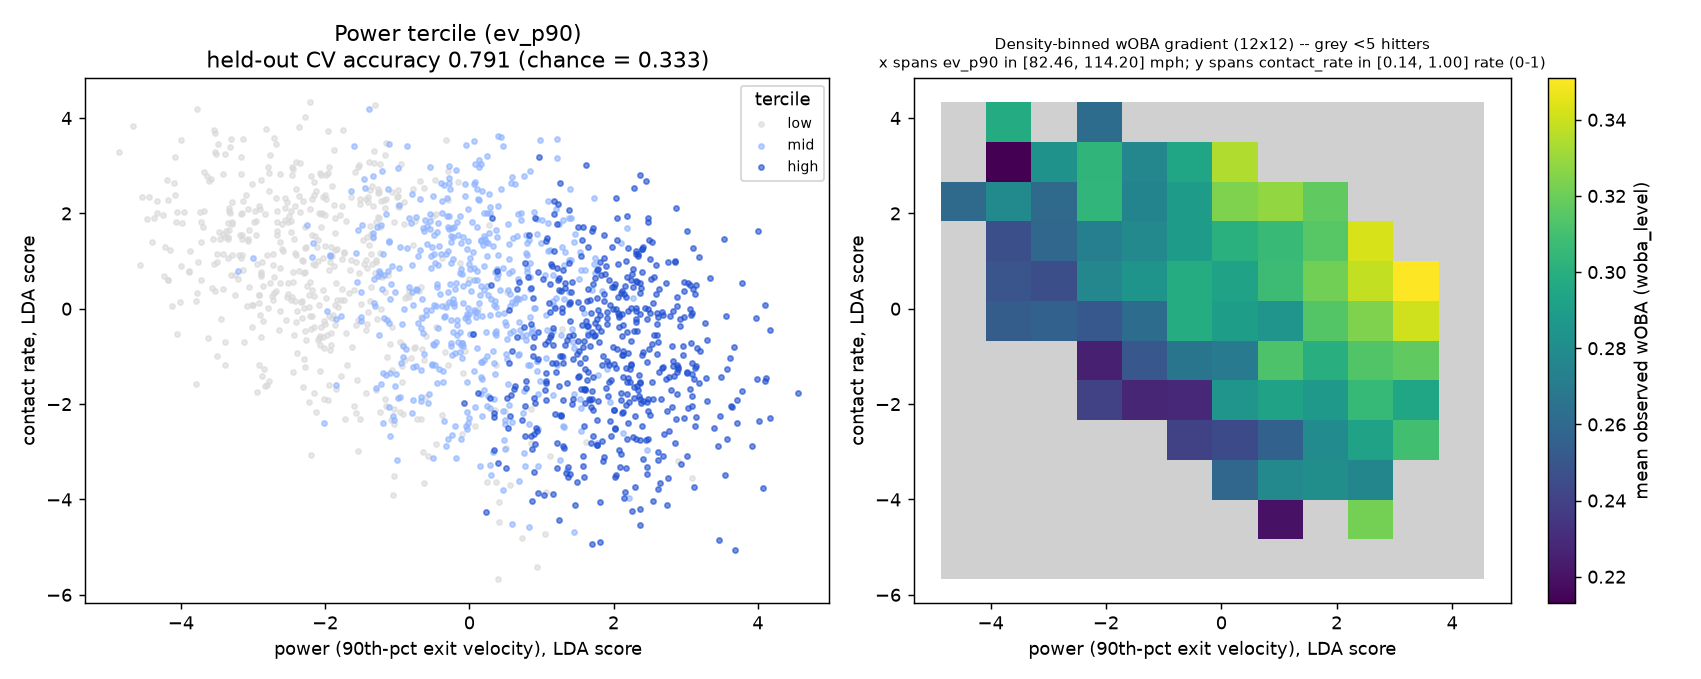
\includegraphics[width=\linewidth]{figs/fig1_power_contact.png}
\caption{Hitters placed by the embedding on fitted power and contact directions. Left: observed power tercile. Right: mean observed wOBA per cell.}
\end{figure}

\section{Conclusion}
The model is better at ordering hitters within a split than at predicting how many points of wOBA the split is worth. For a team, that makes it most useful for ranking platoon options among hitters with a moderate track record, where the decision is actually in question, not as a replacement for a projection system on raw accuracy. Code and processed data: \url{https://github.com/nseluga/hitter-embedding}

\end{document}
